\documentclass[a4j, twocolumn]{jarticle}

%% プリアンブル部 %%
\usepackage{fancybox}
\usepackage{ascmac}
\usepackage[dvipdfmx]{graphicx}

\usepackage{amsmath}
\usepackage{subcaption}

\begin{document}

\title{ゴルフについての基礎知識}
\author{高久　欣也 \thanks{MEKOU}}
\date{\today{}}

\maketitle
\thispagestyle{empty}

\section{ゴルフの誕生}
世界のスポーツの中でも、最も古い歴史を持つと言っても過言ではないのが、"ゴルフ"である.そして,長い歴史を持っているために,その起源はいまだに謎に包まれている.最も有力とされているのは、スコットランドの羊飼いが先の曲がった杖で小石や羊の糞を打ち、ウサギの巣穴へ入れて遊んだのがゴルフにつながったという説である.15世紀にはすでにゴルフが広く多くの人たちの間で楽しまれていた.しかし、

\begin{enumerate}

\item 兵士がゴルフに夢中になり、訓練をおろそかにしたため、イングランドとの戦争に負けた。
\item 国民の多くがゴルフばかりしていて働かなくなった.

\end{enumerate}

などの理由から、1457年、スコットランド王ジェームス2世が、第14議会で「フットボールとゴルフは絶対禁止しなくてはならない.」という、「ゴルフ禁止令」を発令したという記事が残っている~\cite{ref1}.


その後、数回に渡り、「ゴルフ禁止令」が発令された、しかし、1502年当時の国王ジェームス4世が、自分がゴルフをしたかったために、ゴルフ禁止令を解除した.そして人々は再びゴルフを楽しむようになったのである。お隣のイングランドも、この頃にゴルフが伝わったとされている~\cite{ref1}

\section{ゴルフの道具}
ゴルフをするにはなんと行ってもクラブとボールがなければ始まらない.クラブとボールの規格はルールで厳しく制限され、選手は14本のクラブまで使用して良いことになっている~\cite{ref2}.このクラブセッティングが選手の成績に大きく影響する.表1,2に主なクラブの名称、飛距離などを記述する.


\begin{table}[htbp]
    \centering
    \caption{ウッドの説明}
    \label{tab:data1}
\begin{tabular}{|c|c|c|} \hline
    \multicolumn{3}{|c|}{ウッド(Wood)} \\
    \hline
    \hline
    番手 & 名称 & 飛距離 \\ \hline
    1番 & ドライバ & 300 \\ \hline
    2番 & ブラッシ & 280 \\ \hline
    3番 & スプーン & 270 \\ \hline
    4番 & バッフィ & 260 \\ \hline
    5番 & クリーク & 250 \\ \hline
\end{tabular}
\end{table}

\begin{table}[htbp]
    \centering
    \caption{アイアンの種類}
    \label{tab:data2}
\begin{tabular}{|c|c|c|} \hline
    \multicolumn{3}{|c|}{ウッド(Wood)} \\
    \hline
    \hline
    番手 & 名称 & 飛距離 \\ \hline
    1番 & ドライビングアイアン & 250 \\ \hline
    2番 & ミッドアイアン & 240 \\ \hline
    3番 & ミッドマッシー & 230 \\ \hline
    4番 & マッシーアイアン & 220 \\ \hline
    5番 & マッシー & 210 \\ \hline
    6番 & スペードマッシー & 200 \\ \hline
    7番 & マッシー二ブリック & 190 \\ \hline
    8番 & ピッチング二ブリック & 180 \\ \hline
    9番 & 二ブリック & 170 \\ \hline
\end{tabular}
\end{table}

\begin{description}
    \item[ドライバー]
    その昔、材質に柿木（パーシモン）を使用していたことからウッド（wood）とも呼ばれている.心にあたったときは大きな距離が出るが、その反面左右に曲がりやすい.

    \item[フェアウエイウッド]
    ドライバー以外のウッド、最近はアイアンの代わりに利用するゴルファーも多い.片山慎吾がフェアウエイウッドの名手とされている.しかし、ちょっとジジくさい.

    \item[アイアン]
    文字通り（iron）でできている.アイアンと言ってもステンレス、チタンなど固くて軽い材料が利用されている.１番から９番までは番手があるが、アマチュアは１，２，３番アイアンは難しくて使えない.アイアンは距離を合わせる場合やグリーンを狙うときに使われる.

    \item[ウエッジ]
    主にグリーン周りやバンカーに入った球を打つときに使う。距離は出ないが、弾道が高く球が止まりやすい性質がある.ウエッジブランドではボーケイ等が有名.

    \item[バター]
    グリーンに乗った球をカップに沈めるときに使う.とにかくセンスが必要.この一打ちで優勝の行方が変わる.
\end{description}

\section{ドライバーの飛距離}
ドライバーの飛距離はトッププロだと３００ヤードを楽に超える.飛距離はヘッドスピードとクラブの反発係数に依存する.距離をD,ヘッドスピードをS,打ち出し角度を$\theta$,クラブの反発係数をRとすると~\eqref{eq:dist}式のような関係式が成り立つ ~\cite{ref2}.

\begin{equation}
    D = \frac{R \cdot S^2} {\log_{e} 132} \label{eq:dist}
\end{equation}
ちなみに\eqref{eq:dist}式は超テキトーである.

\section{４大メジャーと期待選手}
ゴルフの名誉ある規模最大の大会として以下の４大メジャートーナメントを制して初めて超１流の称号を与えられる.賞金も凄いが,その名誉となると金銭には変えられない価値がある.

\begin{enumerate}
    \item マスターズ
    \item 全英オープン
    \item 全米オープン
    \item 全米プロ選手権
\end{enumerate}
\ref{fig:ref1}にタイガーウッズ(53歳)の写真を掲載する.これまでに,４大メジャー大会を計１５回制覇し、PGA賞金王には10度輝いている.一時期、調子を落とし、2008年以降、メジャー大会での優勝からは遠ざかってしまっていたが、2019年のマスターズで復活優勝を果たした.今年のマスターズでも、持病の影響からスコアを落とし、決勝トーナメントへ出場にはならなかった.

\begin{figure}[htbp]
    \centering
    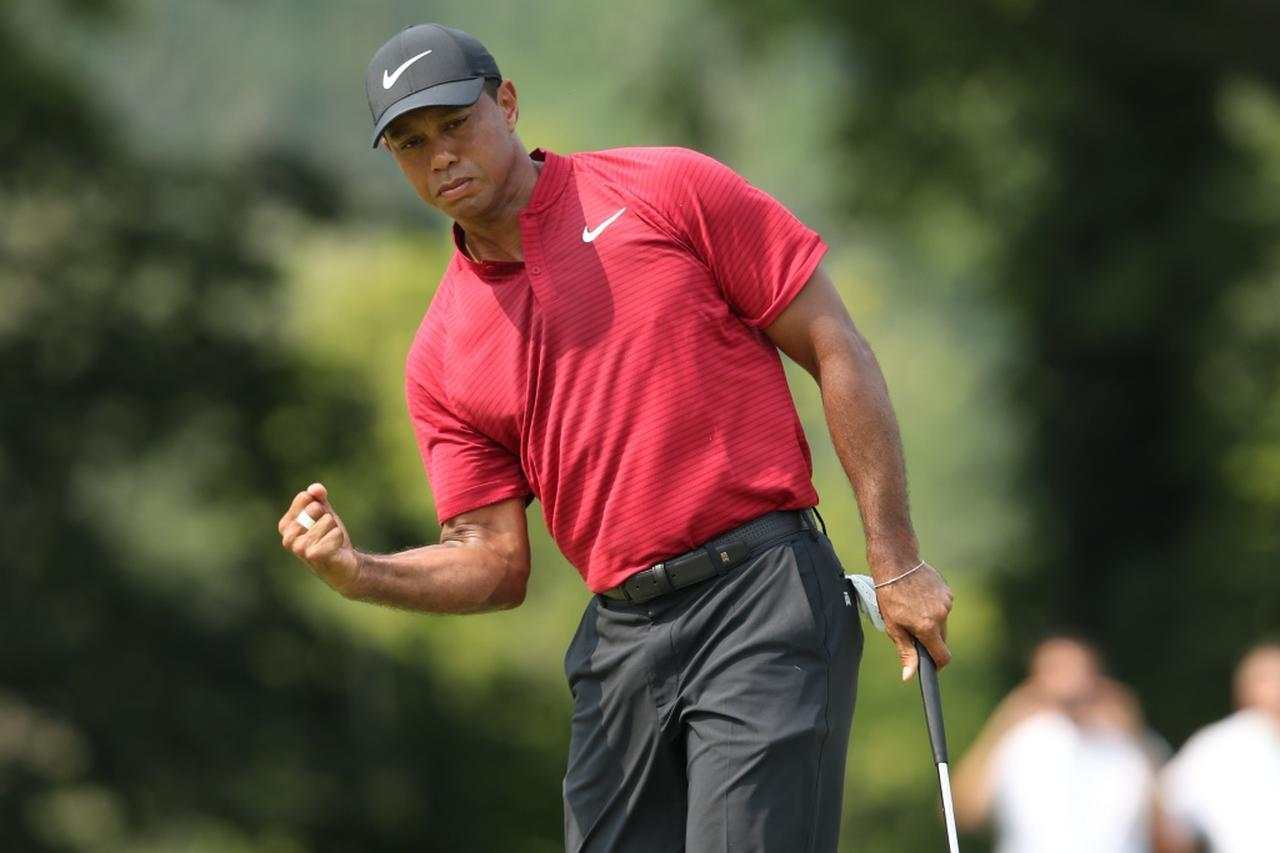
\includegraphics{tiger.jpg}
    \caption{世界の帝王 T. ウッズ}
    \label{fig:ref1}
\end{figure}
図2に活躍を期待される2名の日本人選手を紹介する.


「」は日本のホープ松山英樹選手,2021年度のマスターズでついにアジア人として期待の初優勝を飾る.ずっとメジャー戦優勝を期待できる唯一の日本人としてきたいしてはいたが,今でも信じられないぐらいの快挙である.彼はメンタルも強いが肝心なところでのポカミスがなければ４大メジャー大会制覇も夢ではない.

「」は女子プロの古江彩佳選手,優勝回数はまだ多くはないが、安定した成績で常にランキング上位に位置する実力者である.彼女の特徴は飛距離が全然出ないがコントロールが素晴らしいこと.クラブをぶん回してダイナミックに飛ばす女子プロが多い中で異彩を放つ存在である.

\begin{figure}[htbp]
    \centering
    % 左側の写真
    \begin{subfigure}{0.48\columnwidth}
        \centering
        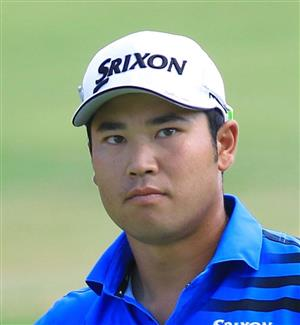
\includegraphics[width=\textwidth]{matuyama.jpg}
        \caption{松山選手}
        \label{sub:matuyama}
    \end{subfigure}
    \hfill % 左右に最大限広げて配置
    % 右側の写真
    \begin{subfigure}{0.48\columnwidth}
        \centering
        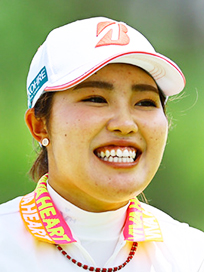
\includegraphics[width=\textwidth]{furue.jpg}
        \caption{古江選手}
        \label{sub:furue}
    \end{subfigure}
    
    \caption{期待の日本人選手}
    \label{fig:japan_players}
\end{figure}
私の期待$\heartsuit$

\begin{thebibliography}{9}
\bibitem{ref1} 穴掘好雄、"俺のゴルフ人生", OB出版,2016
\bibitem{ref2} M. jackson and J. Madonna, "Official Golf \\
Rule", Sports science, 2011
\end{thebibliography}

\end{document}